\section{Conclusions}\label{sec:conclusions}

The methods presented above are implemented in the Python package \texttt{Bayesian\_pyhf} \cite{BayesianPyhf}. This software package enables the parallel Bayesian and frequentist analysis of multi-channel binned models within the single software framework \texttt{pyhf}. \\
The current interface of the package \texttt{Bayesian\_pyhf} is demonstrated in Fig. \ref{code}.
    \begin{figure} %[H]
        \centering
        % \captionsetup{justification=centering}
        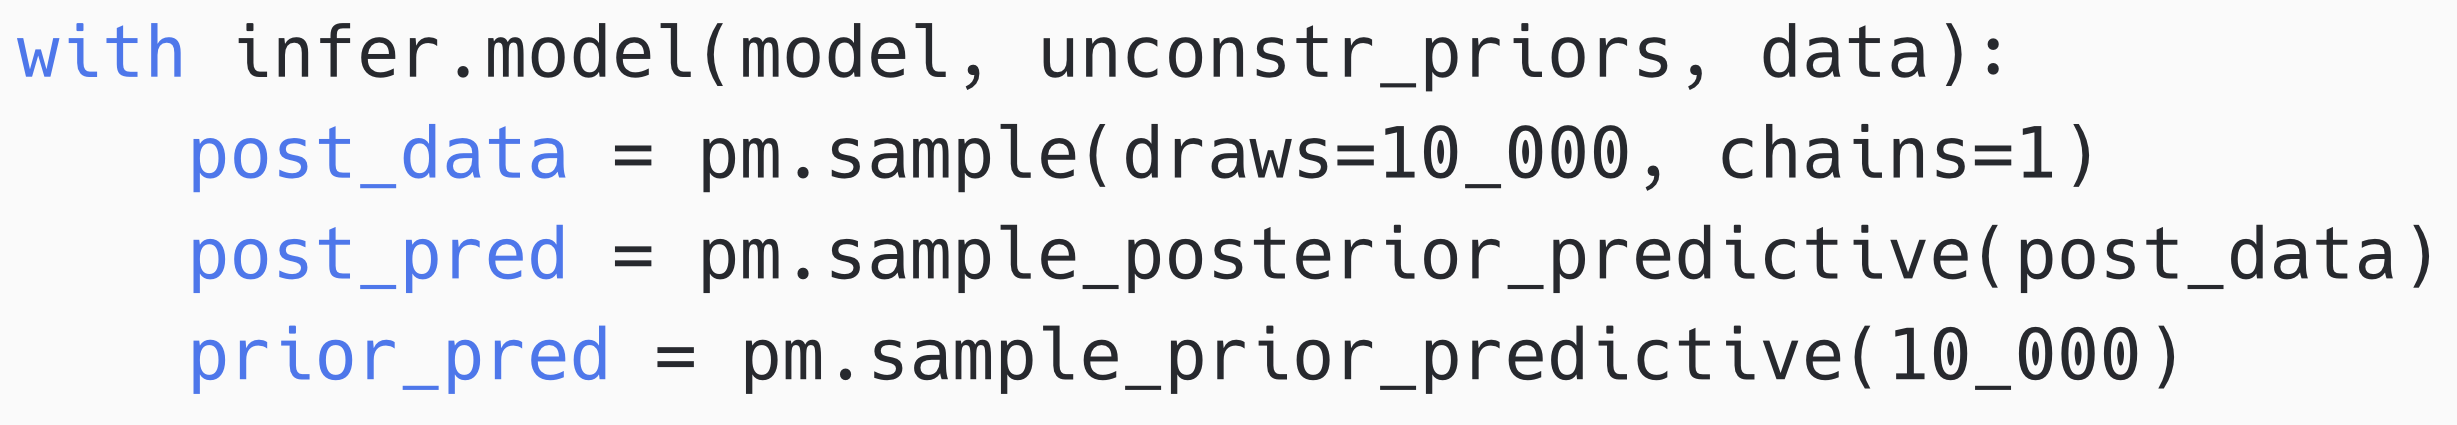
\includegraphics[width=9cm]{figures/code.png}
        \centering
        \caption{Pseudo-code for evaluating \texttt{HistFactory} models using \texttt{PyMC} given some unconstrained parameters and observations.}
        \label{code}
    \end{figure}
\noindent Further enhancements regarding the user interface and stability with respect to multi-chain sampling are ongoing. A full integration in the \texttt{pyhf} is also planned.
